\appendix                     
\section{Technology Models}\label{sec:appendix}
The technology models in Temoa representing energy source are configured with 
data regarding fundamental techno-economic parameters such as their capacity, 
capacity factors, seasonal generation profiles, auxiliary products, waste 
generation metrics, and costs (fixed, capital, variable, and otherwise). 
The following subsections describe the key assumptions about electricity 
generation and storage technologies in the Illinois model built for this 
report.

\subsubsection{Solar Energy Model}
Existing solar power capacities and cost data were averaged over the state and 
based on the \gls{NREL} Annual Technology Baseline for 2020 
\cite{nrel_2020_2020}. However, power 
generation profiles loaded into Temoa representing the variability of solar 
power, such as the seasonal variation in Figure 
\ref{fig:seasonal_hourly_solar}, were derived from a reference solar farm, 
\gls{UIUC} Solar Farm 1.0, located in Champaign, IL. The data was provided by the University of Illinois Facilities and Services Department.
\FloatBarrier

\begin{figure}[H]
	\centering
	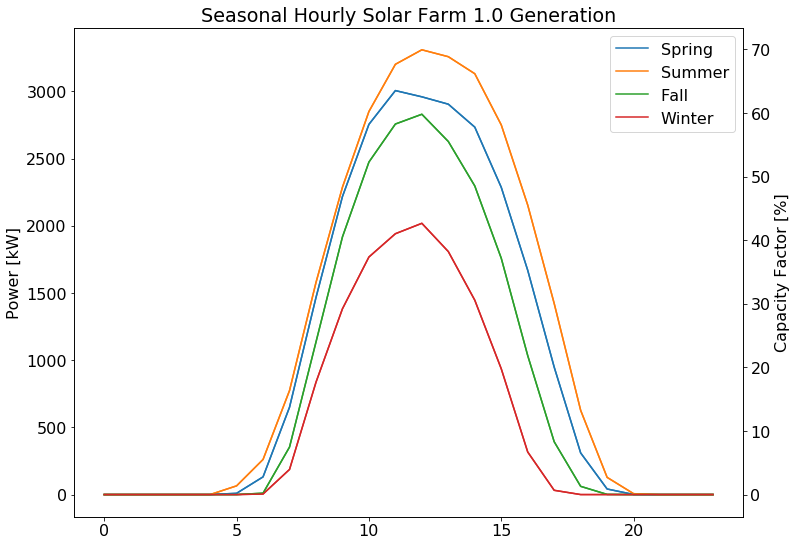
\includegraphics[width=0.7\columnwidth]{./img/seasonal_hourly_solar.png}
	\caption{}
	\caption{The seasonal variation in hourly generation from Solar Farm 
        1.0 at \gls{UIUC}, used as a scaled reference in the Temoa model of the Illinois grid. }
	\label{fig:seasonal_hourly_solar}
\end{figure}

\FloatBarrier

\subsubsection{Wind Energy Model}
Existing wind power capacities, capacity factors, and cost data were averaged over the state and 
based on the \gls{NREL} Annual Technology Baseline for 2020 
\cite{nrel_2020_2020}. However, power 
generation profiles loaded into Temoa representing the variability of wind 
generation, such as the seasonal variation in Figure 
\ref{fig:seasonal_hourly_wind}, were derived from a reference wind farm, Railsplitter Wind Farm, 
located in Lincoln, IL. The data was provided by the University of Illinois 
Facilities and Services Department.
F\&S Department.  \gls{UIUC} has a power purchase agreement with Railsplitter Wind 
Farm.


\begin{figure}[H]
	\centering
	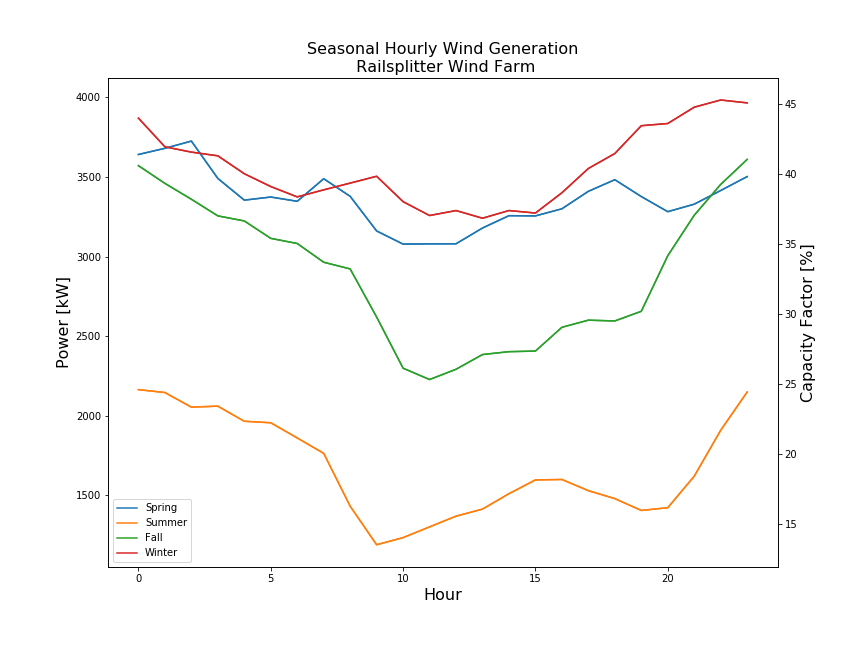
\includegraphics[width=0.7\columnwidth]{./img/cap/seasonal_hourly_wind.png}
	\caption{The seasonal variation in hourly generation from the Railsplitter Wind Farm, used as a scaled reference in the Temoa model of the Illinois grid. }
	\label{fig:seasonal_hourly_wind}
\end{figure}
\FloatBarrier

\subsubsection{Nuclear Energy Model}
Existing nuclear plants in Illinois were specified in the model in accordance with their 
power levels, licensed lifetimes, capacity factors, and costs. Advanced nuclear power plants, 
when available to the model, used pricing from the \gls{NREL} Annual Technology 
Baseline as well as the \gls{NEI} Nuclear Costs in Context report series
\cite{desai_nuclear_2020,desai_nuclear_2018,nrel_2020_2020}.

\subsubsection{Battery Technology}

Grid operators must plan for resource adequacy, and these simulations adopted the standard \gls{NERC} recommendation for planning reserve margin, defined as: 
\begin{align}
         PRM &= \frac{ C_{\text{firm}} - D_{\text{peak}} }{ D_{\text{peak}} }\\
        \intertext{where}
        C_{\text{firm}} &= \text{The firm capacity  [GW]}\nonumber\\
        D_{\text{peak}} &= \text{The peak demand  [GW]}.\nonumber
\end{align}

Firm capacity is sometimes considered the amount of power guaranteed to be
available for the duration of a commitment. We consider firm capacity to be the
amount of power that is available ``on-demand.'' Thus, renewable energy sources
do not contribute to firm capacity. In simulations requiring carbon free
electricity by 2030 in, the only technologies available to contribute to firm
capacity are nuclear power and battery storage. 

\subsubsection{Coal Energy Model}
Coal emissions (NO$_x$, SO$_x$, and CO$_2$) data were retrieved from the 2020 
Sargent and Lundy report, ``Capital Costs and Performance Characteristics for 
Utility Scale Power Generating Technologies'' \cite{sargent__lundy_capital_2020}.

\subsubsection{Natural Gas Energy Model}
Natural gas emissions (NO$_x$, SO$_x$, and CO$_2$) data were retrieved from the 
2020 Sargent and Lundy report on Capital Costs and Performance Characteristics 
for Utility Scale Power Generating Technologies 
\cite{sargent__lundy_capital_2020}.


\subsection{Cost Modeling}

Where available price and cost data could only be found for previous years, we
                accounted for the time value of money by adjusting for
                inflation using the consumer price index from the
                Bureau of Labor Statistics \cite{bls_consumer_2021}. The
                adjusted price becomes:

\begin{align}
        P_{2020} &= \mbox{adjusted price in 2020 dollars }[\$]\\
                &= \frac{P_{n} \cdot CPI_{2020}}{CPI_{n}}\\
        \intertext{where}
        P_n &= \mbox{price in year previous year, n } [\$]\\
        CPI_{2020} &= \mbox{consumer price index for 2020 } [-]\\
        CPI_n &= \mbox{consumer price index for year n } [-].
\end{align}


\subsection{Carbon Pricing of Life Cycle Emissions}
All energy generation technologies have some life cycle emissions.
In order to account for the cost of life cycle carbon emissions from each
technology, a carbon price was applied to the fixed cost of renewables and
nuclear, thus,

\begin{align}
P_c &= \left[\frac{\$}{tCO2}\right] = \left[\frac{M\$}{MTCO2}\right]\\
R_c &= \left[\frac{MTCO2}{GWh}\right]\\\\
FC_c &= R_c\cdot P_c \cdot CF \cdot \frac{hours}{year} = \left[\frac{M\$}{GW-year}\right]
\end{align}

For fossil fuels, this price was included in their variable costs.
